\documentclass[a4paper, 10pt, conference]{ieeeconf}
\usepackage[utf8]{inputenc}
\usepackage{amsmath}
\usepackage{graphicx}
\usepackage{pgf-pie}
\usepackage{tikz}
\usepackage[hidelinks]{hyperref}
\usetikzlibrary{positioning,shadows,arrows,backgrounds}

\usepackage{xcolor}
% \newcommand\todo[1]{\textcolor{red}{\textbf{TODO}: [#1]}}

% \usepackage[disable]{todonotes} % notes not shown
\usepackage[draft]{todonotes}

% \newcommand{\comment}[1]{}  % comment not shown
\newcommand{\comment}[1]{\par {\bfseries \color{blue} #1 \par}} %comment shown

\IEEEoverridecommandlockouts
\overrideIEEEmargins

\title{\LARGE \bf Stegos -- A Platform for Privacy Applications}
\author{The Stegos Team, \today \\v1.0}

\begin{document}

\maketitle
\thispagestyle{empty}
\pagestyle{plain}

%%%%%%%%%%%%%%%%%%%%%%%%%%%%%%%%%%%%%%%%%%%%%%%%%%%%

\begin{abstract}
    In this paper we propose a design for a private, confidential and scalable privacy blockchain that is friendly to the environment. We start with an overview of existing privacy coins, then design a foundation to send payments and data with absolute privacy and complete confidentiality. We extend this foundation to provide a platform for building privacy applications that communicate via messages sent with minimal latency. We describe a Trusted Application Container (TAC), a mobile application that simplifies building privacy applications while providing additional security to users. Last but not least, we sketch the design of an App Store and private marketplaces. 
\end{abstract}

\section{Introduction}
In this section we give a brief overview of most prominent privacy coins and analyze their privacy-protecting and performance characteristics.

We also explain, on a high level, how Stegos builds and improves on existing privacy coin ideas and employs latest research in cryptography and blockchains in order to create privacy-preserving a blockchain that can be scaled. 

\subsection{Terminology}
Here we give definitions for the miscellaneous terms that we are using throughout this paper:

\begin{itemize}
	\item \textbf{Privacy}: protection from detection of the identity of blockchain participants and parties to transactions.
	\item \textbf{Confidentiality}: protection from analyzing blockchain data (e.g. transaction details, including amounts) by unauthorized third parties.
	\item \textbf{Unlinkability}: for any two outgoing transactions it is impossible to prove they were sent to the same person\cite{c2}.
	\item \textbf{Untraceability}: for each incoming transaction all possible senders are equiprobable\cite{c2}.
	\item \textbf{Compactness}: spent coins can be pruned from the blockchain and the blockchain can be compacted.
	\item \textbf{Sharding}: a transaction verification and block-sealing process that can be partitioned between participants or groups of participants.
	\item \textbf{Interactivity}: senders and recipients of transactions must interact with each other \textit{off-chain} before posting a transaction to the blockchain.
	\item \textbf{Trusted Setup}: blockchain participants need to trust someone to generate some initial parameters and then destroy those parameters.
	\item \textbf{PoW}: Proof-of-Work, an original consensus protocol for Bitcoin, where each node participating in the protocol should present a piece of data which is difficult (costly, time-consuming) to produce but easy for others to verify and which satisfies certain requirements. Due to complexity of computations needed and amount of miners, the current energy consumption by Bitcoin PoW consensus is approximately 73TWh per year\footnote{https://digiconomist.net/bitcoin-energy-consumption}.
	\item \textbf{PoS}: Proof-of-Stake is a consensus algorithm, where the creator of the next block is chosen via various combinations of random selection, wealth, age and staked funds. PoS blockchains can be more energy efficient than currencies based on PoS algorithms\footnote{http://cfa-consulting.ch/dlfiles/NxtEnergyandCostEfficiencyAnalysis.pdf}.
	\item \textbf{UTXO}: An Unspent Transaction Output that can be spent as an input in a new transaction.
\end{itemize}

\subsection{Existing privacy coins}

\subsubsection{Monero} originated as a Bytecoin fork in 2014 under the name Bitmonero. The cryptocurrency is using a UTXO model and PoW consensus, and based on the CryptoNote protocol\cite{c2}, employing the ring signatures method. In 2017, Monero implemented RingCT\cite{c3}, an improved version of the ring signatures. RingCT enables confidentiality of amounts and untraceability of transactions. In combination with the stealth addresses (also introduced in the original CryptoNote paper), which provide unlinkability of recipients, this provides full privacy and confidentiality.

Monero's blockchain cannot be compacted because spent UTXOs cannot be pruned from it. Keeping all UTXOs forever is one of the requirements of RingCT protocol, which obfuscates the fact that particular UTXOs mentioned in transaction inputs were actually spent. 
Despite the recent introduction of Bulletproofs\cite{c4} which replaced Monero's original zero-knowledge range proofs and reduced a simple transaction size from 13KB down to 2.5KB, the problem with ever-growing blockchains cannot be solved. 

\subsubsection{ZCash} originated in 2016 as a Bitcoin fork and obviously is using a UTXO model and PoW consensus. The goal of the project is to improve on the flaws of Bitcoin, with a focus on privacy. The project is building on work done on Zerocoin\cite{c5}, addressing some of its faults, like the size of the proofs, which ZCash decreases to 1KB and speeds up the verification.

For establishing confidentiality and untraceability, ZCash implements ``Zero-Knowledge Succinct Non-Interactive Argument of Knowledge'' (zk-SNARKS)\cite{c6}. For providing unlinkability of recipients, ZCash employs stealth addresses.

zk-SNARKS enable a large anonymity set of all minted coins\footnote{The \textit{anonymity set} here defined as the set of participants who could be a sender in ZCash transaction, as seen by a global observer who has also compromised a set of nodes.}, providing a high degree of privacy. However, the size of up to 2KB for an average transaction and ever-growing accumulator, holding serial numbers of all spent coins, that cannot be pruned, makes ZCash much less scalable. The issue of scalability is the main reason why privacy is currently optional, not by default. At the time of writing, less than 25\% of all transactions were shielded.

The questionable part of the zk-SNARKS protocol is the initial trusted setup. ZCash utilizes a multi-party ceremony involving a several trusted people. This is controversial, as you have to trust any of these people that they destroyed the initial parameters and also trust that the ceremony was carried out correctly. 

\subsubsection{Dash} originally a codebase fork from Litecoin (which is in turn a codebase fork of Bitcoin), Dash were launched as XCoin in January 2014. Dash is using the UTXO model and PoW consensus. 

Besides standard nodes and miners, Dash has \textit{masternodes}, the nodes that must have static IP address and fulfill particular requirements for CPU, RAM, and disk space. Each masternode must have at least 1000DASH in its ownership. A Proof-of-Service protocol ensures that masternodes have the most current blockchain protocol and are online. 

It is important to note that privacy is optional in Dash and the high volume of transactions is driven mainly by fast public transactions called \textit{InstantSend} which are provided by masternodes.

\textit{PrivateSend} is an implementation of CoinJoin, the untraceability solution first proposed for Bitcoin by Bitcoin Core developer Gregory Maxwell\footnote{https://bitcointalk.org/index.php?topic=279249.0}. In PrivateSend, three users add their coins together in one big transaction, that sends the coins to freshly generated addresses belonging to the same three users. As such, the coins are effectively mixed between the three participants, breaking the blockchain trail of ownership between them. This process can be automatically repeated up to eight times, with (hopefully) different mixing participants, for extra privacy.

Dash is not providing confidentiality of amounts either in InstantSend, or in PrivateSend. Moreover, it is an essential requirement of CoinJoin protocol that inputs of users involved in the round of the mixing protocol must have exactly the same denomination (amount of coins). This requirement is impossible to fulfill in case of amounts that are cloaked. 

Users of Dash have to trust masternodes that they will keep users' IP addresses undisclosed and unlinked to users' UTXOs when sending transactions in Dash. This adds another privacy vulnerability to Dash.

\subsubsection{Mimblewimble} is a protocol that was proposed by an anonymous user in a Bitcoin developers chat room by the name of Tom Elvis Jedusor, that left a link to a paper\footnote{https://download.wpsoftware.net/bitcoin/wizardry/mimblewimble.txt} in which he outlines that by using the Mimblewimble protocol, the scalability, as well as the privacy of the Bitcoin network, could significantly be enhanced.

Mimblewimble is based on the ideas of Greg Maxwell's design for Confidential Transactions\footnote{https://people.xiph.org/\texttt{\~}greg/confidential\_values.txt}, except, it is the recipient that generates a random blinding factor used to cloak the amount of the transaction. This blinding factor is then used as proof of ownership by the recipient, therefore working simultaneously as the recipient's public key. Therefore, Mimblewimble provides confidentiality of amounts and unlinkability of recipients in its transactions.

Untraceability of transactions in Mimblewimble is building on the ideas of CoinJoin and is implemented by breaking transaction boundaries and storing only inputs and outputs of all transactions verified by miner in a newly mined block.

The two existing implementations of the protocol known at the moment are Grin\footnote{https://github.com/mimblewimble/grin} and Beam\footnote{https://www.beam.mw}. These projects use the UTXO model and PoW consensus. Spent UTXOs in both projects can be pruned by recursively applying a simple pruning algorithm for each UTXO referenced in inputs of the new minted block.

There are several drawbacks in the design of Mimblewimble:

\begin{itemize}
	\item {The first drawback is related to the transaction creation mechanism of MimbleWimble --- in order to create a transaction, senders and recipients must interact with each other. The sender cannot post a transaction to the blockchain without first contacting the recipient with half-baked transaction data and receiving that data updated by applying a blinding factor back from the recipient.}
	\item {The second is very similar to the problem from Dash where users must trust Dash masternodes. Currently, Grin and Beam users must trust miners that they will not trace the history of inputs and outputs in transactions, and discard this data completely after mining a block. Therefore, there is a threat to the coins' fungibility and the privacy of users.}
\end{itemize}

\subsection{Our contribution}
In this paper we propose a design for \textit{Stegos}, a blockchain which uses the \textit{UTXO} (coin) model and \textit{PoS} (Proof-of-Stake) consensus.

\subsubsection{Absolute privacy}
Transactions in Stegos are \textit{unlinkable}, \textit{untraceable}, and \textit{confidential}:

\begin{itemize}
	\item {Stegos uses one-time payment addresses which make it impossible to identify recipients of a transaction, e.g. to link addresses of recipients to their identities, because all transactions are directed to new and unique addresses. The technique we use for one-time addresses is very similar to stealth addresses used in Monero and ZCash.}
	\item {Stegos makes it impossible to trace the history of transactions since many individual transactions are pooled together to form a super-transaction. For this purpose, we adopted and enhanced the ValueShuffle protocol\cite{c7}, the first coin mixing protocol compatible with Confidential Transactions.}
	\item {All amounts in Stegos are hidden using Pedersen commitments\cite{c8} and Bulletproofs (range proofs)\cite{c4}. Validator stakes and transaction fees are the only exception since these must be visible for blockchain validation.}
\end{itemize}

\subsubsection{Data compaction}
Many projects claim to be able to process a million transactions per second (TPS) but none of them explain how they are going to maintain all the accumulated data. Bitcoin provides for 7--10 TPS and the Bitcoin blockchain is expected to grow past 170 gigabytes by the end of 2018. If we assume that Bitcoin suddenly supports 16,000 TPS, the Bitcoin blockchain will grow by 350 gigabytes every day\footnote{https://hackernoon.com/if-we-lived-in-a-bitcoin-future-how-big-would-the-blockchain-have-to-be-bd07b282416f}, or 127 terabytes every year. This amount of data is completely unsustainable unless the blockchain will be centralized on a few supercomputers, something that’s contrary to blockchain’s decentralization ethos.

\subsubsection{Transactional sharding}
Stegos is a \textit{compact} blockchain. Spent coins are safely removed from the blockchain using secure cryptographic pruning. To keep our blockchain free of spent coins, we are using the technique proposed originally by Satoshi Nakamoto in the Bitcoin paper\cite{c1}.

Stegos uses transactional \textit{sharding} to scale. Separate groups of Stegos validators keep the whole blockchain state but verify only a subset of incoming transactions, using cross-shard atomic commits to eliminate double-spending. This scalability approach enables Stegos process thousands of transactions per second.

\subsubsection{Proof-of-stake (PoS)}
Stegos is friendly to the environment and does not require terawatts of electricity to be spent for mining blocks. Stegos uses PoS (Proof-of-Stake) consensus, building on ideas of pBFT\cite{c9} and Collective Signing\cite{c10}\cite{c11}. Each new Stegos block must be verified and confirmed by a group of validators, all of which must put a performance bond or stake.

The size of the coins staked has a direct effect on the probability of a validator becoming the leader of a consensus round and earning block rewards and transaction fees.
\todo[inline]{Talk about mobile staking}

\subsubsection{Fast data messaging}
\todo[inline]{Describe data messaging in a nutshell}

\subsubsection{Trusted Application Container (TAC)}
\todo[inline]{Describe the purpose of the TAC}

\subsubsection{Additional incentives}
Stegos includes a couple of additional incentives to drive adoption and encourage viral marketing. 

\textit{Jackpot} is a feature unique to Stegos and a lottery concept that everyone is familiar with. A portion of the fees from each block are added to the Jackpot and any stake forfeited by a validator caught cheating goes into the Jackpot as well. 

Users create \textit{tickets} with their lucky numbers and post them to the blockchain. The Jackpot is distributed every few thousand blocks when validators run a cryptographic lottery based on verifiable distributed randomness to generate the winning number. Several tiers of prizes are awarded depending on how closely the ticker numbers match the winning number. 

\textit{Red envelopes}\footnote{https://en.m.wikipedia.org/wiki/Red\_envelope\#Digital\_red\_envelopes} is a WeChat-like feature that we implement to promote viral growth. Users create red envelopes with a given number of tokens and post the corresponding QR code or URL on social networks. Each attempt to open the red envelope may result in a few tokens or none at all. 

In the following sections we will explain each of the Stegos features in more detail.

\section{Networking}\label{Networking}

The Stegos network is composed of \textit{bootstrap nodes}, \textit{compact nodes} and \textit{light wallets}. Bootstrap and compact nodes maintain a copy of the blockchain and associated data structures. They post a performance bond (stake) to become \textit{validators}, then participate in the consensus protocol and earn block rewards, as well as transaction fees. These nodes also respond for request from light wallet nodes.

Bootstrap nodes carry the unpruned version of the blockchain and respond to bootstrap requests new compact and bootstrap nodes. Compact nodes carry the pruned version of the blockchain, i.e. the current UTXO set.

\todo[inline]{What are our incentives for bootstrap nodes?}
\todo[inline]{How do we verify that bootstrap nodes carry the full blockchain data?}

Light nodes only keep blockchain headers and know how to talk to validators. 

Stegos will initially maintain the core of the network by running a number of validator nodes to ensure continuity and performance of the network. The addresses of the core nodes will be hard-coded into each release of the Stegos blockchain software.

Nodes keep a list of addresses of the nodes they know about (peers) and add new peers to the list as they become aware of them. A brand new node will connect to one of the core nodes to fetch a list of bootstrap nodes and download a copy of the blockchain. 

Each full node quickly re-broadcasts received transactions to a subset of its peers, after a few  light checks. This both ensures that a node cannot be DDOS-ed with transactions to validate and that it does not re-broadcast junk transactions.

To discourage bad actors, we employ a mechanism to both throttle peers and punish peers for bad transactions, e.g. by blocking them from further participation in the network.

The Stegos blockchain uses a gossip protocol to spread information without depending on a fixed network topology. This protocol does not require every node to be reliable or always up and running, and does not require every node to know about every other node. Each node knows about just a few peers and information can safely propagate through the network as long as most nodes know of at least two peers.

\section{Randomness}\label{Randomness} 

Bias-resistant distributed randomness is a critical component of Stegos. We employ \textit{RandHound++}, our own, improved variant of RandHound\cite{c12}, a large-scale distributed protocol that provides publicly-verifiable, unpredictable, and unbiased randomness by implementing an efficient and decentralized randomness beacon. The protocol arranges participants into verifiably unbiased random secret-sharing groups, which repeatedly produce random output at predefined intervals. 

We use RandHound++ for multiple purposes:

\begin{itemize}
	\item {to form validator groups;}
	\item {to elect leaders of validator groups;} 
	\item {to choose pooled transactions facilitators among validators;}
	\item {to find a winner of the Jackpot lottery.}
\end{itemize}

See Appendix \ref{RandomnessAppendix} for more details of our randomness implementation. 

\section{Consensus}\label{Consensus}

The Stegos consensus protocol is based on pBFT\cite{c9} but adds strong consistency, which enables all validators to agree on the validity of blocks without wasting computational power resolving inconsistencies. Clients do not need to wait more than a few seconds to be certain that a submitted transaction is committed; as soon as it appears in the blockchain, the transaction can be considered confirmed.\todo[inline]{A few seconds? Confirm this!}

\subsection{Collective Signing}
We adopt \textit{CoSi}\cite{c10}\cite{c11}, a scalable witness cosigning protocol ensuring that every authoritative statement is validated and publicly logged by a diverse group of witnesses before any client will accept it. A statement $S$ collectively signed by $W$ witnesses assures clients that $S$ has been seen, and not immediately found erroneous, by those $W$ observers. Even if $S$ is compromised in a fashion not readily detectable by the witnesses, CoSi still guarantees $S$’s exposure to public scrutiny, forcing secrecy-minded attackers to risk that the compromise will soon be detected by one of the $W$ witnesses. 

CoSi builds on existing cryptographic multi-signature methods, scaling them to support thousands of witnesses via signature aggregation over efficient communications. The default implementation of CoSi uses Schnorr signatures which we replace with BLS signatures for performance reasons.

Please see the Appendix \ref{ValidationAppendix} for more details on how we use CoSi to sign blocks.

\subsection{Leader Election}
Stegos is a public so anyone can join the network, become a validator and earn rewards for maintaining the blockchain. Stegos uses Proof-of-Stake (PoS) consensus and all validators need to post a performance bond (stake). Requiring a performance bond helps against Sybil attack by requiring a significant financial commitment from validator.\todo[inline]{There must be a better way to say this}

Any validator caught cheating by their peers loses their stake, which gets transferred into the Jackpot. 

A validator elected to become the leader of the current epoch is rewarded by collecting transaction fees from the blocks they form, as well as collecting the block reward. 

Leader election is done using a stake-weighted lottery. The larger the validator's stake, the greater the chances of becoming the leader of the current consensus round (epoch). After serving as the leader of one epoch, the leader relinquishes his right to be re-elected until a number of rounds later.

Please see Appendix \ref{ConsensusAppendix} for the exact details of our consensus protocol.

\section{Transactions}\label{Transactions}

In previous sections, we explained the high-level concepts of Stegos, including networking, randomness, and consensus. Now it is time to describe the inner details of Stegos, such as the composition of its coins and basic transactions.
\todo[inline]{Give a high-level overview of transactions}

\section{Snowball}\label{Snowball}
\todo[inline]{Give a high-level overview of our ValueShuffle implementation}

\subsection{A problem of establishing untraceability}
Even though user identities are cloaked in the blockchain, the spending history of every UTXO can be established by tracing blockchain transactions backwards, up to the genesis block.

Despite having a serious hurdle for such tracing --- we don't store transactions in the blocks of out blockchain, but rather Merkle trees of inputs and outputs --- a malicious node may join our network right after mainnet release, to collect transaction history in order to analyze and trace UTXOs.

To counteract this, we want to implement a protocol that completely hides the relationship between inputs and outputs of each transaction. This is difficult because UTXOs must have a unique $ID$. Without such a unique $ID$ there's no way to validate transactions or prove ownership of a UTXO. Unique UTXO $ID$ establish a trail which we want to obscure by only showing that UTXO output could have come from one of many different and unrelated inputs. We want to hide the source of each UTXO but in a manner that allows public validation.

\subsection{Possible solutions}
Currently there are four kinds of approaches for solving the problem of establishing untraceability: coin mixers, Ring Signatures, zk-SNARKs, and the CoinJoin family of protocols.

\subsubsection{Mixers} require that users trust the third-party which provides mixing services, something that's unacceptable in a truly private and confidential blockchain.

\subsubsection{Ring Signatures} collect a large but random number of existing UTXOs and add those into the list of inputs actually being spent. A signature is formed on all of the inputs, enabling proof that the inputs are properly spent as a group, without revealing the exact inputs being spent. 

Ring signatures prevent blockchain compaction since it's impossible to know if a UTXO becomes spent and prune it from the blockchain. All UTXOs \textit{that ever existed} must be retained which does not scale very well.

\subsubsection{zk-SNARK} stands for ``Zero-Knowledge Succinct Non-Interactive Argument of Knowledge.'' Currently, the only known way to produce zero-knowledge proofs that are non-interactive and short enough to publish to a block chain is to have an initial setup phase that generates a common reference string shared between prover and verifier. Anyone with access to the secret randomness used to generate the reference string is able to create false proofs that will look valid to the verifier. For a cryptocurrency that uses zk-SNARKs, e.g. Zcash, this means creating counterfeit coins. 

To prevent double-spending in a zk-SNARK-based cryptocurrency, a cryptographical accumulator has to be maintained by all nodes and contain the serial numbers of all spent coins. This accumulator always grows and cannot be trimmed, which scales poorly.

\subsubsection{CoinJoin} is a protocol for joining several Bitcoin transactions together before submitting them to miners to include in the block. The protocol was originally proposed by Greg Maxwell in 2013 and is based on the following idea: ``When you want to make a payment, find someone else who also wants to make a payment and make a joint payment together.''\footnote{https://en.wikipedia.org/wiki/CoinJoin} CoinJoin implementations are based on the usage of trusted servers that provided the service of mixing multiple transactions together.

In 2014, CoinJoin inspired researchers from Saarland University to develop a completely decentralized protocol they called \textit{CoinShuffle}\cite{c17}. It also allows users to mix their coins with those of other interested users and uses the accountable anonymous group communication protocol \textit{Dissent} to ensure anonymity and robustness against DoS attacks. 

The same researchers presented an enhanced version of the protocol in 2016, which they called \textit{CoinShuffle++}\cite{c18}. The key innovation of CoinShuffle++ is replacing mix-nets with Dining Cryptographers Networks (DC-nets)\cite{c20}, a more efficient anonymity mechanism. 

A mix-net requires sequential processing so the number of communication rounds in the original CoinShuffle protocol grows linearly with the number of users. By using DC-nets, CoinShuffle++ allows for mixing to proceed in parallel, requiring a constant number of communication rounds regardless of the number of users. 

\subsection{ValueShuffle}
We improve on \textit{ValueShuffle}\cite{c19}, an extension of CoinShuffle++ that is compatible with confidential transactions. ValueShuffle ensures the anonymity of mixing participants as well as the confidentiality of their payment values, even against malicious mixing participants. The ValueShuffle paper is missing some key details, though. For example, the paper provides neither details on forming a pool of senders who wish to mix their transactions, nor the details on how to form a signature on the resulting pooled transaction. 

We implement a protocol where a \textit{facilitator} elected among the validators provides the services of the \textit{Bulletin Board} (as defined in the ValueShuffle protocol). We also implement collective Schnorr signatures\cite{c22} on the resulting transaction. Details of these protocols, as well as a brief explanation of our implementation of ValueShuffle, are given in Appendix \ref{SnowballAppendix}.

\section{BlockCrunch}\label{Pruning}

As described in Appendix \ref{Block}, a Stegos block is composed of a header and a body, where the header contains root hashes of two Merkle trees, that comprise the body of the block. Those two trees are a tree of all inputs (TXIN Merkle Tree) and a tree of all outputs (TXOUT Merkle Tree). 

When a new block is verified and signed by CoSi witnesses, the signatures are computed over just the block header. The body of the block is not signed because it is secured against modification by the nature of the Merkle tree. It will be impossible to modify the body of the block without invalidating the root hashes contained in the signed header.

After verifying and signing a new block, the \textit{leader} broadcasts it to the network. All nodes must validate the collective block signature and process the new block using the following steps:

\begin{itemize}
	\item {A node must retrieve all leaves of TXIN Merkle Tree from the block body, and for each leaf (UTXO $ID$) do the following:
	\begin{enumerate}
		\item {Find the block that contains the UTXO with $ID$}
		   \item {Find a leaf in the TXOUT Merkle Tree of that block that contains the UTXO}
		\item {Mark the leaf as \textit{SPENT} without modifying the value of the hash that belongs to that leaf}
		\item {If a sibling leaf is also marked as \textit{SPENT} then delete \textit{both leaves and their corresponding hashes}. Then mark the parent node of these two pruned leaves as \textit{SPENT} as well and restart from step 4. Repeat until there are no \textit{SPENT} siblings left.}
	\end{enumerate}} 
	\item {If the process above applies to all UTXOs in the TXIN Merkle Tree of the block, delete that tree from the block body and leave just the TXIN Root Hash in the block header. Append the block to the local copy of the blockchain.}
\end{itemize}

Stegos blockchain compaction is a continuous process where each incoming and properly signed block triggers the pruning. As a result of this continuous pruning, the Stegos blockchain becomes a database of unspent coins (UTXO), with no transaction history kept.

\section{FastData}\label{FastData}

The Stegos blockchain can be used for sending and temporarily storing arbitrary data payloads. 

\todo[inline]{Describe data messaging}

\section{Tokenomics}\label{Tokenomics}
\todo[inline]{Write an introduction to our tokenomics}

\subsection{Block rewards and transaction fees}\label{BlockRewardsAndFees}
\todo[inline]{Describe block rewards and transaction fees}

\subsubsection{Inflation}\label{Inflation}
\todo[inline]{Describe inflation}

\subsection{Jackpot}\label{Jackpot}
\todo[inline]{Describe the Jackpot}

\subsection{Red packets}\label{RedPackets}
\todo[inline]{Describe the red packets}

\section{The privacy platform}\label{PrivacyPlatform}
\todo[inline]{Introduce the need for privacy apps}

\subsection{Issues with existing apps}
\todo[inline]{Talk about unscrupulous developers stealing coins}

\subsection{The Trusted Application Container}\label{TAC}
\todo[inline]{Describe the TAC}

\subsection{Example apps}
\todo[inline]{Describe one-on-one and group chat}

\subsection{Marketplaces}
\todo[inline]{Describe marketplaces}

\subsection{The Privacy App Store}
\todo[inline]{Describe the App Store}

\section{Future work}\label{FutureWork}
\todo[inline]{Describe the future roadmap}

\subsubsection{Mobile staking}\label{MobileStaking}
\todo[inline]{Describe mobile staking}

\section{Next Steps}

In this paper we laid out a design for Stegos - a private, confidential, and scalable blockchain that is eco-friendly, upon which applications for sending monetary values and/or arbitrary data can be built.

The Stegos team is working on implementation of the blockchain and the development progress can be tracked online at \url{https://github.com/orgs/stegos/projects/1}. Our source code is and always be 100\% open.

As our implementation progresses, we will publish separate, more detailed papers focused on our most essential contributions to the blockchain ecosystem, like improved distributed randomness generation (\textit{RandHound++}), our flavor of collective signing protocol and consensus based on it (\textit{BLS CoSi/pBFT}), and our approach for transactions and data sharding. 

\begin{thebibliography}{99}

\bibitem{c1} Satoshi Nakamoto. ``Bitcoin: A Peer-to-Peer Electronic Cash System,'' https://bitcoin.org/bitcoin.pdf, October 31, 2008.

\bibitem{c2} Nicolas van Saberhagen. ``CryptoNote v 2.0,'' https://cryptonote.org/whitepaper.pdf, October 17, 2013.

\bibitem{c3} Shen Noether, Adam Mackenzie and Monero Core Team. ``Ring Confidential Transactions,'' https://lab.getmonero.org/pubs/MRL-0005.pdf, February, 2016.

\bibitem{c4} Benedikt Buenz, Jonathan Bootle†, Dan Boneh, Andrew Poelstra, Pieter Wuille, and Greg Maxwell. ``Bulletproofs: Short Proofs for Confidential Transactions and More,'' Cryptology ePrint Archive, Report 2017/1066, 2017. URL: https://eprint.iacr.org/2017/1066.

\bibitem{c5} I. Miers, C. Garman, M. Green and A. D. Rubin. ``Zerocoin: Anonymous Distributed E-Cash from Bitcoin,'' 2013 IEEE Symposium on Security and Privacy, Berkeley, CA, 2013, pp. 397-411. URL: https://ieeexplore.ieee.org/document/6547123

\bibitem{c6} Nir Bitansky, Ran Canetti, Alessandro Chiesa, and Eran Tromer. 2012. ``From extractable collision resistance to succinct non-interactive arguments of knowledge, and back again,'' in Proceedings of the 3rd Innovations in Theoretical Computer Science Conference (ITCS '12). ACM, New York, NY, USA, 326-349. URL: https://dl.acm.org/citation.cfm?id=2090263

\bibitem{c7} Tim Ruffing and Pedro Moreno-Sanchez. ``Mixing Confidential Transactions: Comprehensive Transaction Privacy for Bitcoin,'' Cryptology ePrint Archive, Report 2017/238, 2017. URL: https://eprint.iacr.org/2017/238

\bibitem{c8} Torben Pryds Pedersen. ``Non-Interactive and Information-Theoretic Secure Verifiable Secret Sharing,'' Advances in Cryptology --- CRYPTO '91", Springer Berlin Heidelberg, 1992, pages 129--140.

\bibitem{c9} Miguel Castro and Barbara Liskov. ``Practical Byzantine Fault Tolerance,'' Proceedings of the Third Symposium on Operating Systems Design and Implementation, 1999, pages 173--186. 

\bibitem{c10} Ewa Syta, Iulia Tamas, Dylan Visher, David Isaac Wolinsky, Philipp Jovanovic, Linus Gasser, Nicolas Gailly, Ismail Khoffi, Bryan Ford. ``Keeping Authorities “Honest or Bust” with Decentralized Witness Cosigning,'' arXiv:1503.08768v4 [cs.CR], 30 May 2016. URL: https://arxiv.org/pdf/1503.08768.pdf

\bibitem{c11} Eleftherios Kokoris-Kogias, Philipp Jovanovic, Nicolas Gailly,
Ismail Khoffi, Linus Gasser, and Bryan Ford. ``Enhancing Bitcoin Security and Performance with Strong Consistency via Collective Signing,'' arXiv:1602.06997v3 [cs.CR], 1 Aug 2016. URL: https://arxiv.org/pdf/1602.06997v3.pdf

\bibitem{c12} Ewa Syta, Philipp Jovanovic, Eleftherios Kokoris Kogias, Nicolas Gailly, Linus Gasser, Ismail Khoffi, Michael J. Fischer, Bryan Ford. ``Scalable Bias-Resistant Distributed Randomness,'' Cryptology ePrint Archive, Report 2016/1067, 2016. URL: https://eprint.iacr.org/2016/1067.

\bibitem{c13} Ignacio Cascudo, Bernardo David. ``SCRAPE: Scalable Randomness Attested by Public Entities,'' Applied Cryptography and Network Security, Springer International Publishing, 2017, pages 537--556.

\bibitem{c14} Youliang Tian, Changgen Peng, Renping Zhang, Yuling Chen. ``A practical publicly verifiable secret sharing scheme based on bilinear pairing,'' 2nd International Conference on Anti-counterfeiting, Security and Identification, IEEE, 2008.

\bibitem{c15} M. Stadler. ``Publicly verifiable secret sharing,'' in Advances in Cryptology--EUROCRYPT ’96, volume 1070 of Lecture Notes in Computer Science, pages 190--199, Berlin, 1996. Springer-Verlag.

\bibitem{c16} Dan Boneh, Ben Lynn, Hovav Shacham. ``Short Signatures from the Weil Pairing, '' Journal of Cryptology", 2004, volume 17, pages 297--319.

\bibitem{c17} Tim Ruffing, Pedro Moreno-Sanchez, Aniket Kate. ``CoinShuffle: Practical Decentralized Coin Mixing for Bitcoin,'' University of Saarland, Germany, 2014. URL: http://crypsys.mmci.uni-saarland.de/projects/CoinShuffle/coinshuffle.pdf

\bibitem{c18} Tim Ruffing, Pedro Moreno-Sanchez, Aniket Kate. ``P2P Mixing and Unlinkable Bitcoin Transactions,'' University of Saarland, Germany, 2016. URL: https://crypsys.mmci.uni-saarland.de/projects/FastDC/paper.pdf

\bibitem{c19} Tim Ruffing, Pedro Moreno-Sanchez. ``Mixing Confidential Transactions: Comprehensive Transaction Privacy for Bitcoin,'' Cryptology ePrint Archive, Report 2017/238, 2017. URL: https://eprint.iacr.org/2017/238

\bibitem{c20} David Chaum. ``The dining cryptographers problem: Unconditional sender and recipient untraceability,'' Journal of Cryptology", 1988, volume 1, pages 65--75.

\bibitem{c21} Whitfield Diffie, , Martin E. Hellman. ``New Directions in Cryptography,''   in IEEE Transactions on Information Theory, volume 22 (6), pages 644--654. 

\bibitem{c22} C.P. Schnorr. ``Efficient Identification and Signatures for Smart Cards,''
in Advances in Cryptology --- CRYPTO' 89, 1990, Springer, pages 239--252.

\end{thebibliography}

\appendices

\section{Randomness}\label{RandomnessAppendix}

\subsection{Distributed Randomness Generation}
The idea of performing distributed randomness generation is to have many nodes participate in the construction of an untainted and unpredictable random value in order to overcome Byzantine faults which might try to steer, or predict, the outcome.

RandHound++ is based on the notion of publicly verifiable secret sharing (PVSS)\cite{c15}, which ensures that every step of the process can be audited using zero knowledge proofs (ZKP), while keeping vital details of the process fully cloaked through strong cryptography.

But unlike distributed Consensus Protocols, like pBFT, we do not need full Byzantine threshold participation at every stage. In what follows we assume a maximum number, $f$, of faulty nodes, in a collection of $(3 f + 1)$ participant nodes. 

The usual Byzantine Fault Tolerance (BFT) requires responses from a super-majority of $(2 f + 1)$ nodes in order to reach consensus. But in our application, generating randomness, as long as at least one honest participant blends its randomness into the computation, the result will be purely random. We do not need consensus on the result as long as its process can be verified.

Hence we only need $(f + 1)$ responses from participants to overcome any Byzantine faults, where at least one participant will be honest, and supplies true randomness. There is no need for consensus on the actual value generated. It is sufficient to see only that at least one node was honest. That is clearly true with $(f + 1)$ participants. Attackers can perturb the final value, but it will still become an honest random value by virtue of the inoculation property.

\subsection{RandHound++}
Our variant of the RandHound protocol is implemented with pairing-based cryptography (PBC). As such, it departs in a number of significant ways from the original RandHound algorithm. It is a distributed protocol for generating audit\-able, untainted, and unpredictable randomness, as required for fair stake-weighted elections of the validator group leader, among the other purposes.

After every election, a validator group's \textit{leader} is selected, and then a \textit{beacon} node is chosen among the remaining validators. The \textit{beacon} node is responsible for partitioning all validators (including itself and the \textit{leader} into RandHound++ groups. 

The first validator in any group becomes a local group leader who collects randomness from all its group members and itself, and then forwards that result back to the \textit{beacon}. The \textit{beacon} then combines all the group randomness values into a single result that becomes the seed value for the next elections, then the \textit{beacon} sends a \textit{HOLD-ELECTION} message, with that seed value, to all validators in the network.

A major advantage of PBC is that we can use efficient BLS signatures\cite{c16} in the protocol. Such signatures can be collectively added, along with the group sum of their public keys, to produce a short collective-signature that can be validated just as easily as a single signature. BLS signatures are efficient because multi-signatures can be generated immediately and do not require a second query from participants in order to produce their collective signature.

But PBC entails some complications in translating the RandHound algorithm to asymmetric pairs of elliptic curves. Though these complications are purely conceptual --- the mathematics are more difficult. But PBC performs nicely, with the same efficiencies for producing PVSS data as are to be had with producing BLS signatures.

We will publish a separate paper describing in more detail our improvements on the original RandHound protocol in the nearest future.

\section{Consensus}\label{ConsensusAppendix}
In order to produce a stake-weighted lottery, we could imagine dividing a circle into angular sections proportional to individual stakes, with the full circumference of the circle representing the sum of all stakes. A uniformly generated random number over a finite interval (this is where our RandHound++ protocol comes in handy) acts as a spinner in a dial readout, and wherever it points after a spin, that member is selected as the next leader. Larger stakeholders occupy a larger portion of the circumference, and have a better chance of winning.

\begin{figure}[h!]
\centering

\resizebox{.3\textwidth}{!}{%

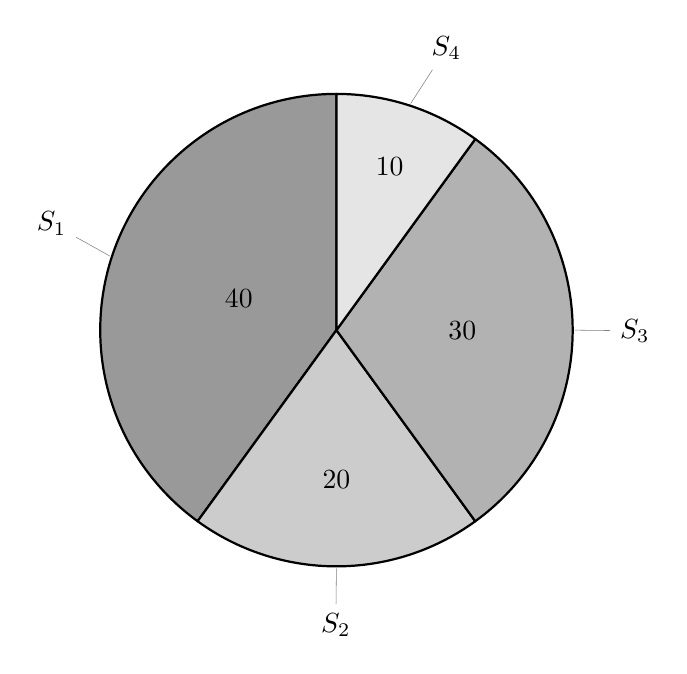
\begin{tikzpicture}
\pie [text=pin, rotate = 90, before number =, after number =,
	  color={black!40,black!20,black!30,black!10}]
	{40/$S_{1}$, 20/$S_2$, 30/$S_3$, 10/$S_4$}
\end{tikzpicture}

}%

\bigskip

\resizebox{.3\textwidth}{!}{%
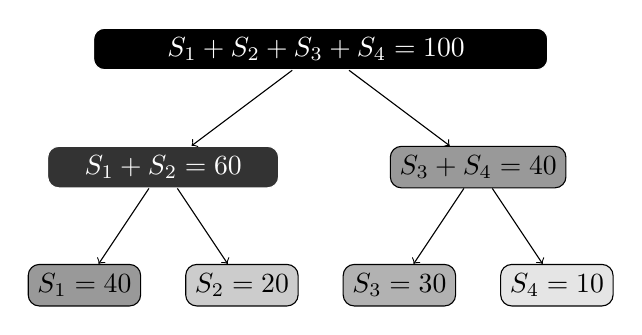
\begin{tikzpicture}[sibling distance=4cm,
  every node/.style = { shape=rectangle, rounded corners,
	draw, align=center, top color=white, bottom color=blue!20}]

\node[color=white, top color=black!100, bottom color=black!100]
	 {\ \ \ \ \ \ \ \( S_1 + S_2 + S_3 + S_4 = 100 \) \ \ \ \ \ \ \ }
	 child[->]
		  { node[color=white, top color=black!80, bottom color=black!80]
				{\ \ \ \( S_1 + S_2 = 60 \)\ \ \ }
				child[sibling distance=2cm]
					 { node[top color=black!40, bottom color=black!40] {\( S_1 = 40 \)}}
				child[sibling distance=2cm]
					 { node[top color=black!20, bottom color=black!20] {\( S_2 = 20 \)}}
		  }
	 child[->]
		  { node[top color=black!40, bottom color=black!40]
				{\(S_3 + S_4 = 40 \)}
				child[sibling distance=2cm]
					 { node[top color=black!30, bottom color=black!30] {\( S_3 = 30 \)}}
				child[sibling distance=2cm]
					 { node[top color=black!10, bottom color=black!10] {\( S_4 = 10 \)}}
		  };
\end{tikzpicture}
}%

\caption{Imagining a spin dial as a tree. Segments
are sized in proportion to the posted stake.}
  \label{fig:spinner}
\end{figure}

In practice, we form a binary tree of participants, in a consistent order, where each interior node represents the sum of all its sub-node stakes. The topmost node of the tree shows the full sum of all stakes represented in the tree, with all participants located in leafs. Branching decisions begin at the top node of the tree and descend toward leafs. This is done using the random value as a probe of the interval described by the partial sum at each node. The division between left and right are based on the relative weights of its two subtrees. Descent continues until meeting a leaf node, and declaring that node the winner of the leader election. 

If the random probe value is converted into a fractional value of its range, and each interior node is re-labeled with this fractional value, then it is simple to choose between left or right subnodes based on a single comparison between two fractional values.

We can see that this works by noting that every interior node of the tree serves both as a denominator to nodes below, and as a numerator to connections above, hence cancelling out completely. The final probability of any participant winning becomes the size of their stake divided by the sum of all participating stakes.

\subsubsection{Handling leader election failures} 
Leader elections are held on a schedule and validators recognize the signal to hold a new election. 

The list of validators is publicly known and can be re-built by processing staking transactions starting with the genesis block. Validators keep a number of data structures in memory, including the list of other validators, and update these data structures when accepting blocks to add to the end of the chain.

Each validator can re-run the election for themselves upon seeing the random value of the election signal, which arrives via RandHound++ protocol. All nodes should be able to agree on election outcome, but if not, then one of two things could happen: 

\begin{itemize}
	\item{First, if a validator thinks it won the election but was mistaken, then any attempts at forming new Cosi networks by the faux leader will be silently rejected by others, and it will fail to obtain a consensus on any new requests. If that happens, the rejected leader will re-synchronize its list of validators, rerun its own election, and re-join after agreeing on the outcome.} 
	\item{Second, a validator may think that someone else had won the election. In that case, it will silently reject signing requests by actual election winner, and never see any requests from the presumed one. The validators will re-sync its list of other validators if this happens for two consecutive election rounds.}
\end{itemize}

If the election winner is absent or comes under attack, it may not respond to its own election as leader, form the block, or broadcast the block for signing. Any validator can call for a new early election, and after $(2 f+1)$ (supermajority) of such calls from different validators have been seen, a new election round will start.

\subsubsection{A fault-tolerant and self-healing protocol} 
Immediately after a leader election, each validator should determine its role for the new epoch:

\begin{itemize}
	\item If elected leader, then begin next block assembly. 
	\item If the node should become a member of a RandHound++ group, then start running the protocol within its group.
	\item If the node should become a facilitator for the transaction pooling protocol, then start collecting transaction intent messages.
	\item If the node should become a CoSi witness node, then start a timeout timer. If that timeout ever fires, then it is time to call for a new election. Incoming messages can restart or cancel the timeout timer, though.
	\item Otherwise, the node is on standby for the next election cycle. Nodes on standby can ignore almost all messages, but must pay attention to election-related messages.
\end{itemize}  

All validators should pay attention to leader election messages:

\begin{itemize}
	\item{\textit{New Election Message}: run an election with the random value provided in the election message, and determine next role for this validator --- one of leader, witness signer, RandHound++ participant, facilitator, or standby. Reset the counter of calls for new election.}
	\item{\textit{Call For New Election Message}: Increment the count, $n$, of such calls seen from different validators, and if $n \ge 2 f +1$, then run another election round based on the last election's random value, with a decision tree that excludes current leader. Determine new leader and next role for this validator. Reset the counter of calls for new election.}
\end{itemize}

\subsection{Key Blocks}

Stegos blockchain is able to accommodate multiple kinds of blocks. The kind of the block is defined by the \textit{Block Type ID} slot in the block header. In this paper we define two types of blocks: $0 (KeyBlock)$ and $1 (MonetaryBlock)$.

Monetary blocks, the blocks that carry all cryptocurrency transactions data and coins, will be described in detail in Section \ref{block}. We will be referring to them simply as \textit{blocks} throughout this paper. 

The purpose of Key blocks is to deliver the administrative information to blockchain participants. Any node, searching through key blocks, can see who is current or past epoch \textit{leader}, and who are witnesses (validators) for the current or past epoch. Nodes wishing to submit a transaction should consult with the latest key block to find who is the current pooled transactions \textit{facilitator}.

The key block header is constructed by the current \textit{leader} filling in the following slots:

\begin{itemize}
	\item {Block Type ID, 0}
	\item {Version Number}
	\item {Epoch Number}
	\item {Previous block hash, computed as the hash of the block header of the current blockchain tip block}
	\item {\textit{Leader} public key}
	\item {Ordered list of witness public keys; the leader node is also considered a witness}
	\item {Pooled Transactions \textit{facilitator} public key}
	\item {BLS Multi-signature, to be filled in as a result of the consensus on the block.}
	\item {Bitmap of signers in the multi-signature}
\end{itemize}

There is no body in the key block.

The initial contents of the BLS Multi-signature slots should be zero filled and, even after being filled in, never contribute to the computation of any \textit{block header hash}. All other slots are concatenated to form a header hash pre-image.

The key block verification and sealing should be done using the same consensus protocol as for the monetary blocks. We will describe this protocol in detail later on in this paper, in Section \ref{block}.

\section{Basic Transactions}\label{TransactionsAppendix}

In previous sections, we explained the high-level concepts of Stegos, including networking, randomness, and consensus. Now it is time to describe the inner details of Stegos, such as the composition of its coins and basic transactions.

\subsection{UTXO Structure}\label{UTXO}

For illustrative purposes, suppose that some coins have been sent from Alice to Bob. Alice's public key is $P_A$, while Bob's secret key is $s_B$ and his public key is $P_B$. To help preserve anonymity, all public keys in Stegos are cloaked with a random value chosen from a very large finite field, $Z_r$.

When Alice sends coins to Bob, she cloaks their amount with a Pedersen commitment, which is both binding and hiding. It binds Alice to her commitment so that she can never alter the amount of coins. The commitment also hides the amount from the general public, while simultaneously providing proof to the public that the amount is legitimate. Only Alice and Bob know how many coins are being transferred. 

\subsubsection{Pedersen commitment and Bulletproof} To form a Pedersen commitment, Alice multiplies the amount by a generator, $A$ for the Elliptic curve group, $E_r$, of prime order $r$. To that, she cloaks the commitment by adding a multiple, $\gamma$, of the publicly known generator point, $G$, with the multiple being chosen randomly from the finite field, $Z_r$. Generators $A$ and $G$ must have no known relationship. Placing the cloaking factor on the main generator curve will become important as we proceed. This is the same curve which holds all public keys. 

The Pedersen commitment is thus:
$$ C(x, \gamma) = x \, A + \gamma \, G \in E_r$$
$$x, \gamma \in Z_r$$

where $x$ denotes the number of coins being transferred, $A$ is the amount-curve generator, and $G$ is the principal generator. We denote the commitment by $C(x, \gamma)$. 

This commitment value will be wrapped inside a Bulletproof range proof on the amount, $x$, which also proves that the amount lies within a legitimate range of values, typically a 64-bit number.

\subsubsection{Destination address cloaking} Alice then cloaks Bob's public key with a factor, $\delta \in Z_r$, so that instead of Bob's original public key $P_B$, she will put into UTXO $P_{B, \delta} = P_B + \delta \, G$.


\subsubsection{Encrypted payload} Alice must pass values for the amount $x$, and cloaking factors, $\gamma$ and $\delta$, to Bob. She can do it by including this information into the \textit{encrypted payload} of the UTXO. Besides the values mentioned above, the encrypted payload may also contain arbitrary data, that Alice wants to share with Bob. Detailed explanation of storing arbitrary data on Stegos blockchain will be given in Section \ref{data}. 

For generating the encrypted payload, Alice must choose random values $\alpha, k \in Z_r$ that will be used in creating and cloaking a symmetric data encryption key.
The actual symmetric key for the encrypted data object will be $H(k \, G)$. In order to pass it safely via the blockchain to Bob, Alice needs to cloak it with $\alpha$ and store it in the UTXO as the following tuple: $$\mathit{Key}_{\alpha} = (\alpha \, P_{B} + k \, G, \alpha \, G )$$ 

Alice encrypts her payload with AES-128 using $H(k \, G)$ key and places the encrypted payload into the UTXO as $E_B(x, \gamma, \delta)$.

When Bob receives UTXO later on, he will take out $\mathit{Key}_{\alpha}$ from it, multiply the second element of the tuple by his secret key $s_B$, getting $s_B \, \alpha \, G = \alpha \, P_B$, then subtract that from the first element to find $k \, G$. Afterwards he produces $H(k \, G)$ thus computing the symmetric key and decrypts the payload that Alice sent to him.

\subsubsection{TTL and Data Size} Alice sets TTL (time-to-live) and $Size_{data}$ slots of the UTXO to zero, indicating that this is a \textit{monetary UTXO}. Non-zero values of the mentioned slots will indicate that this is \textit{data UTXO}, handling of which will be described in details later in this document, it Section \ref{data}.

\subsubsection{UTXO ID} Alice forms a UTXO $\mathit{ID}$ by hashing the the whole UTXO object sans the ID slot, which contains the cloaked version of Bob's public key, $P_{B, \delta}$, the Pedersen commitment and Bulletproof, TTL, $Size_{data}$, and the encrypted payload.

The UTXO $\mathit{ID}$ becomes a unique identifier, since, if all else were equal, the $\gamma$ and $\delta$ factors were randomly chosen from field $Z_r$.

\subsubsection{UTXO structure}

Thus the resulting structure of the UTXO object will be the following:

\begin{multline*}
UTXO = (ID, P_{B, \delta}, Bp, TTL, Size_{data},\\
        Key_{\alpha}, E_B(x, \gamma, \delta))
\end{multline*}

where

\begin{align*}
ID &= H(P_{B, \delta}, Bp, TTL, Size_{data}, \\ 
   & Key_{\alpha}, E_B(x, \gamma, \delta)) \in Z_r \\
H(arg_1, arg_2, ...) &= \textit{hash mapping of concat args} \\
P_{B, \delta} &= P_B + \delta \, G \\
G &= \textit{known generator for group } E_r \\
Bp &= \textit{Bulletproof and Pedersen} \\
& \textit{commitment on amount}, x 
\end{align*}

\begin{align*}
TTL &= \textit{Time-to-Live}, 0 \\
Side_{data} &= \textit{Data payload size}, 0 \\
Key_{\alpha} &= (\alpha \, P_{B} + k \, G, \alpha \, G ) \\
E_B(x, \gamma, \delta) &= \textit{AES-128 encrypted payload}
\end{align*}

Nowhere is either of Alice's or Bob's public key shown. We only present a cloaked version of Bob's key. And since $\delta$ is a secret value, nobody can recover the actual public key underlying the cloaked version. 

Therefore Bob may publish his public key openly, i.e. on his website or in an invoice, and need not worry that his identity will be linked to the recipient of the payment on Stegos blockchain, because his public key will appear in Stegos UTXOs always in a cloaked from -- every time as a completely new and random number.

\subsection{Transaction Structure}

When Bob wants to spend his new tokens, he must form a transaction containing a list of inputs (TXINs) and outputs (TXOUTs). TXINs are nothing more than the $\mathit{ID}$s referring to other UTXOs. TXOUTs are a list of new UTXOs. He must also offer a valid signature on the entire transaction, which simultaneously proves his ownership of all TXIN's, proves that the transaction carries zero net balance of funds between TXINs, TXOUTs and fees, and protects the contents of his transaction against mutation by MITM attackers.

A UTXO can only be spent in its entirety, and if it carries excess value for his purposes, he will produce a TXOUT with change back to himself, thereby creating a new UTXO. Bob must show that the sum of all inputs to his transaction equals the sum of all outputs plus fees. He can do so with Pedersen commitments so that his transaction is binding on him, while also disclosing nothing about the actual amounts involved.

To form his signature, he adds together all the $\delta$ cloaking factors from the UTXOs specified by his TXINs list of $\mathit{ID}$s, adds in all the $\gamma$ cloaking factors from the Pedersen commitments in the Bulletproofs from those same UTXOs, and subtracts the $\gamma$ cloaking factors used in his own TXOUT UTXOs. 

Suppose Bob uses $N$ TXINs. His own public key, $P_B = s_B \, G$. Then his effective secret key for the signature becomes:
$$s_{\mathit{eff}} = N \, s_B + \sum_{i \in \text{ins}} {\delta_i} + \sum_{i \in \text{ins}}{\gamma_i} - \sum_{j \in \text{outs}}{ \gamma_j}$$

Using this effective secret key, he produces a Schnorr signature pair, $(u, K)$, after choosing $k \in Z_r$ at random:
$$K = k \, G$$
$$u = k + H_r(K, P_{eff}, H(T)) \, s_{\mathit{eff}}$$
$$Sig(s_{eff},T) = (u, K)$$
so that validators can see that:
$$u \, G = K + H_r(K, P_{eff}, H(T)) \, P_{eff}$$
$$P_{\mathit{eff}} = \sum_{i \in \text{ins}}{P_i} + \sum_{i \in \text{ins}}{C_i} - \sum_{j \in \text{outs}}{C_j} - \mathit{Fee} \, A$$
where $T$ represents the entire transaction record, sans signature. The function $H_r(x)$ represents the hash $H(x)$ mapped onto the field $Z_r$.

Let's examine the commitment terms. Pedersen commitments are additively homomorphic:
$$C(x_1, \gamma_1) + C(x_2, \gamma_2) = C(x_1 + x_2, \gamma_1 + \gamma_2)$$

Hence, if Bob's transaction is valid, the amount terms in the effective public key show a zero balance on the $A$ curve, after subtracting off the $\mathit{Fee}$. What remains is entirely on the $G$ curve. The validator sum becomes another public key on the $G$ curve, exactly matching his own computed effective secret key, $s_{\mathit{eff}}$. Only Bob could form a valid signature since it relies on his secret key. It is unforgeable. Both Alice and Bob know all the other secret items, $\gamma$'s and $\delta$'s. Nobody else knows any of the secret values.

Suppose Bob now just wants to send the coins he received from Alice on to Charlie, after deducting fees. In that case, Bob forms a UTXO that uses a different blinding factor, $\gamma_2$, and different key cloaking value, $\delta_2$, and which contains amount, $(x - \mathit{Fee})$. Bob must form a new Bulletproof on the amount, and encrypt these values into a payload that only Charlie can read:

\begin{multline*}
ID' = H(P_{S, \delta_2}, Bp', TTL, Size_{data}, \\
          Key_{\alpha_2}, E_S(x - Fee, \gamma_2, \delta_2))
\end{multline*}

where $P_{C, \delta_2}$ is Charile's cloaked public key for this transaction, $TTL$ and $Size_{data}$ are zero, and $Key_{\alpha_2}$ is a cloaked symmetric key. 

Charlie can spend this UTXO by providing a valid transaction signature against the UTXO \textit{ID'}, just like Bob did for his own input. 

Bob's TXOUT will now look like this:

\begin{multline*}
\text{TXOUT} = (ID', P_{S, \delta_2}, Bp', TTL, Size_{data},\\ 
                Key_{\alpha_2}, E_S(x - Fee, \gamma_2, \delta_2))
\end{multline*}

To wrap up, Bob publishes the transaction:

\begin{align*}
\text{T} = \{&\text{TXIN} : \{\mathit{ID}\}, \\
 &\text{TXOUT} : \{(ID', P_{S, \delta_2}, Bp', TTL, Size_{data}, \\
 & \ \ \ \ \ \ \ \ \ \ \ \ \ \ Key_{\alpha_2}, E_S(x - Fee, \gamma_2, \delta_2))\}, \\
 &\text{FEE} : \mathit{Fee}, \\
 &\text{GAMMA} : \gamma_{\mathit{adj}} = \sum_{i \in \text{ins}}{\gamma_i} - \sum_{j \in \text{outs}}{\gamma_j}\\
 &\text{SIG} : \mathit{Sig}(s_B, T)\}
\end{align*}

The first line is Bob's TXIN referencing the UTXO produced for him by Alice. The second line is the TXOUT - a new UTXO aimed at Charlie. The third line shows the fees paid for this transaction, in clear text form. 

The fourth line shows what value of $\gamma$ adjustment, on the $G$ curve, is needed to see that the sum of input commitments equals the sum of output commitments, proving a zero net balance between TXINs and TXOUTs and Fee. And this term will be added to a block sum when the transaction is absorbed into the blockchain, to show that entire blocks, which may contain many UTXOs, continue to show a zero balance.

The final line is Bob's signature asserting ownership of the entire transaction which is based on the hash of all the stated TXINs, TXOUTs, $Fee$, and $\gamma_{adj}$ term. This final signature also serves as a checksum against mutation of the contents of this transaction. If anything becomes changed in this record, the signature won't check. Hence our transactions are non-malleable.

\section{Snowball}\label{SnowballAppendix}

\subsection{Forming the pool of senders}
Each epoch, besides selecting new witnesses, a leader, and a winner of the Jackpot, all validators select a node among them which must serve as a \textit{Bulletin Board} in ValueShuffle protocol and include the public key of this node into the sealed keyblock for the new epoch. We call that Bulletin Board node \textit{a facilitator}.

Each node intending to submit a transaction should broadcast a \textit{Transaction Intent} message with a fresh ephemeral public key along with the signature proof of validity.

\textit{Facilitators} should listen to transaction intent messages from the nodes and pool public keys from those messages into collections of $K$ keys each. $K$ defines a cardinality of the anonymity set by defining how many participants should form a transaction mixing pool. This is a tunable parameter which can be set for an each epoch of the blockchain. 

Upon collection of $K$ keys or on the timeout of $T$ seconds, \textit{the facilitator} broadcasts \textit{Transactions Pool} message (signed with its private key), containing all collected ephemeral public keys and corresponding signatures.

Each node that recognizes its key in \textit{Transactions Pool} messages should sort the collection of keys from it in ascending numerical order, form the hash of the collection, and use that hash as a random seed for the \textit{Pooled Transactions Session}.

\textit{A pool leader} is elected by participating nodes by forming the XOR of the hash value defined above with the public key of the each pool participant and, if the resulting value is the minimum in the list, then that node should be chosen as a \textit{pool leader}.

\textit{A pool leader} is responsible for publication of a final pooled transaction, that we call a \textit{super-transaction}.

\subsection{Establishing the pooled transaction session}
All communications, including broadcasting, within the pooled transactions session should be contained within the group of the pool participants. All nodes of the pool will broadcast their lists of TXINs along with signatures validating ownership of their TXINs. Every participant can validate the lists from other participants by verifying the signature attesting to TXIN ownership. Participants should check that the public key referenced by the TXIN $ID$ is from one of the group members.

\subsubsection{Collecting inputs} 
A valid signature on the TXINs from one participant is formed by creating a Schnorr signature on the sum of the cloaked public keys shown in the UTXOs referenced in the TXINs:

\begin{align*}
TXIN &= \{ID_1, ID_2, ..., ID_N\}\\
Sig &= (u, K)\\
K &= k \, G \\
s_{cmp} &= N s + \sum_i{\delta_i}\\
P_{cmp} &= N P + (\sum_i{\delta_i})\, G = s_{cmp} \, G\\
u &= k + H_r(K, P_{cmp}, H(ID_1, ID_2, ..., ID_N)) \, s_{cmp},
\end{align*}

where the sum is over the list of TXINs, $s$ is the owner's secret key, $P = s \, G$ is the corresponding public key, and the $\delta_i$ are the cloaking factors used on the public key of the owner. $N$ refers to how many TXINs there are in the list. Value $k$ is chosen randomly from the field, $Z_r$. 

Verification of a signature is done by seeing that:
$$u \, G = K + H_r(K, \sum_i{P_i}, H(ID_1, ID_2, ..., ID_N)) \, \sum_i{P_i}$$
where the $P_i$ are the cloaked public keys shown in the UTXOs corresponding to each $ID_i$. This signature proves ownership of the stated UTXOs referenced in TXINs.

Nothing in this broadcast identifies the sender, but one cannot count on that to hold. In the event of misbehavior, a blame cycle will require each node to submit all their shared secret keys, which effectively reveals their full transactions. A restart will compute new TXOUTs, so that a successful run ensures anonymity of participants. But if a blame cycle is performed, there is no way to cloak the associations to TXINs again.

Once contributions have been received from each participant, or a timeout occurs, the resulting pool of TXINs is known to all participants. Since these are merely UTXO $ID$s pointing into the immutable blockchain, no further changes can occur to this list except for removal of individual TXIN references as some participants are found to go offline during the protocol, or else when a cheater is detected and then excluded for a restart of the protocol.

\subsubsection{Establishing pair-wise shared keys} 
All participants will establish pair-wise shared secret keys between themselves and every other participant of the pooled transactions session. These shared keys are used to form cloaking factors in the anonymizing protocol, such that, only after pooling results from all participants will the collection of data shared among them become apparent. Until that time, all information remains cloaked. After that time, the data will be known, but no associations can be inferred regarding who supplied which portions of the data. 

It is important to the protocol, that between any two users both of them are using the same shared secret cloaking key. Only then will the sum of all cloaking factors, from all participants, cancel out in the DiceMix arrays. But users are prevented from seeing each other's secrets since the total cloaking factor also sums contributions related to all other participants, and those keys are unknown to the other party.

Shared keys can be securely established between every pair of participants using a Diffie-Hellman secure key exchange\cite{c21}. With two participants, $A$ and $B$, this can be established by having $A$ send to $B$
$$A \rightarrow B: (\alpha \, P_B, Sig(P_A))$$
for $\alpha$ randomly chosen by $A$, and where $Sig(P_A)$ securely authenticates this information as having come from $A$. The signature includes the public key, $P_A$. 

Then $B$ responds to $A$ with
$$B \rightarrow A: (\beta \, P_A, Sig(P_B))$$
with $\beta$ being chosen randomly by $B$. 

After the exchange, the shared key is a hash of the product:
$$key = H(\alpha \beta \, G)$$ 

But since neither side knows both factors, at $A$ we compute:
$$\beta \, G = (\beta \, P_A) / s_A$$
since $P_A = s_A \, G$. And at $B$ we compute
$$\alpha \, G = (\alpha \, P_B) / s_B$$
Then each side can multiply their result by their chosen randomness to reveal $(\alpha \beta \, G)$. Nobody watching the exchange can deduce the shared secret key.

\subsubsection{Producing DiceMix arrays for outputs} 
Next, each participant computes their TXOUTs with \textit{fresh randomness}, chooses random $k$-factors for an eventual collective Schnorr signature, and produces both a DiceMix array containing the fragmented TXOUTs, and cloaked running sums of their $\gamma_{adj}$ and $K$-signature values. The hash commitment of this information is signed and broadcast to all participants. This commitment will be used to verify information during the following passes to verify that information was properly transmitted.

The DiceMix array contains successive powers of TXOUTs fragments, cloaked with self-canceling seeds that zero-out after all participants pool their results from the next pass. After forming the DiceMix array and running sums, this information is signed and broadcast to all participants. Anonymity is assured because of the DiceMix cryptographic mixing process. Even though all participants can see, from the accompanying signature, who delivered a DiceMix array, they cannot see which components of the collection were contributed by any participant. The entire collection is revealed only after summing the DiceMix arrays from all participants.

The individual $K$-signature terms from each participant are summed in a blind sum. We do this to prevent combinatorial exploration, once signature $u$-values are disclosed, which could lead to associations between TXINs and TXOUTs.

\subsubsection{Forming the super-transaction} 
On receipt of all DiceMix arrays and the running sums, each participant can form the polynomial, using Newton's Identities, whose roots are the individual contributions. Solving that polynomial for its roots reveals each component of participants' TXOUTs. These TXOUTs are reassembled, and a \textit{super-transaction} is formed containing all TXINs, TXOUT's, the $\gamma_{adj}$ sum needed to show zero balance, and the $K$-signature sum needed for a collective Schnorr signature.

Each participant validates the entire transaction for correctness by examining the $\gamma$ sums for zero balance, and verifying the TXOUTs Bulletproofs. They must also find their own contributions in the lists of TXINs and TXOUTs. If the super-transaction does not properly validate, then someone has cheated, and we enter a \textit{blame discovery cycle}. Otherwise we proceed to the formation of the collective signature. 

\subsubsection{Forming the collective Schnorr signature} 
Knowing the super-transaction, and the collective $K_{sum}$ signature term, each participant broadcasts their $u$-signature component to be summed with those of other participants, yielding a collective Schnorr signature on the whole super-transaction.

Signature formation on the super-transaction for each participant is done as follows:

\begin{align*}
T &= \text{super-transaction} \\
Sig_i &= (u_i, K_{sum}) \\
K_{sum} &= \sum_i{k_i \, G} \\
s_{cmp,i} &= N \, s_i + \sum_{j \in \text{ins}} {\delta_j} + \sum_{j \in \text{ins}} {\gamma_j} - \sum_{k \in \text{outs}} {\gamma_k} \\
P_{cmp,i} &= s_{cmp,i} \, G \\
P_{sum} &= \sum_i{P_{cmp,i}}\\
u_i &= k_i + H_r(K_{sum} , P_{sum},  H(T)) \,  s_{cmp,i}\\
\end{align*}

where index $i$, labels each participant, index $j$, labels every TXIN, for $N$ of them, belonging to the participant, and index $k$, labels each TXOUT belonging to that participant. On summation from all participants, the multi-signature $(u_{sum}, K_{sum})$ represents a valid signature on the super-transaction in the same manner that would hold if this were a simple transaction.

\subsubsection{Publishing the super-transaction} 
At the end of this final signature pass, each participant should have a super-transaction that can be validated by public witnesses. But all connections between TXINs and TXOUTs will have been broken. All that anyone can see is that all TXINs are being spent, and each TXOUT must have derived from one or more of those TXIN, but no way to see which ones are associated. \textit{The session leader} then sends the super-transaction into the network using gossip protocol for validation and inclusion into the block.

\subsubsection{The blame cycle} 
If a blame cycle must happen, each participant must divulge their shared secret keys. Then all other nodes can verify that all stages of the computation were performed correctly, according to the information sent previously. We then have known associations between TXINs and TXOUTs. Any participant which cannot or will not do this is blamed for the fault, and the protocol restarts after taking note of the TXINs associated with the cheating node.

But since secret shared keys were divulged during blame discovery, all participants must restart the protocol from the point of establishing new shared keying.

\section{Validation of Blocks and Transactions}\label{ValidationAppendix}

\subsection{Validation of Transactions}
On entry to the witness pool, a transaction needs to be validated. The steps are:

\begin{itemize}
	\item{For each TXIN, a witness must locate the UTXO referred to by the $ID$, to find the public key, Bulletproof, and Pedersen commitment, used for signature formation. If any $ID$ does not point to an existing UTXO, then the entire transaction is invalid.}
	\item{No two TXINs can point to the same UTXO, to prevent double-spend attempts.}
	\item{All of the cloaked public keys must be summed, along with all of the Pedersen commitments from the TXINs. Then all of the Pedersen commitments from the Bulletproofs in the TXOUTs must be subtracted from the sum, as well as $Fee$ times the $A$ curve generator. The Schnorr signature in the transaction must be checked against this summed public key:

	\begin{align*}
		\text{TXINs} &= \{ID_1, ID_2, ..., ID_N\} \\
		ID_i &\rightarrow P_{i, \delta_i} = P_i\\
		ID_i &\rightarrow C(x_i, \gamma_i) = C_i\\
		P_{eff} &= \sum_{i \in \text{ins}}{P_i} + \sum_{i \in \text{ins}}{C_i}  - \sum_{j \in \text{outs}}{C_j} - Fee\,A\\
		Sig(s, T) &= (u, K)\\
		T &= \text{Entire transaction sans signature}
	\end{align*}

	Now check that
	$$u \, G = K + H_r(K, P_{eff}, H(T)) \, P_{eff}$$
	
	If this equation holds true, then the transaction body has not been mutated, the sender has proven ownership of all UTXOs referenced in the TXINs, and the transaction represents a proper zero balance.}
	\item{The Bulletproofs in every TXOUT must be validated to ensure that amounts are within proper range, that no money is being created on credit.}
\end{itemize}

At this point, we now have a valid transaction to consider. Commitments are held inside each Bulletproof.

The paired TXINs and their UTXOs must be marked as pending extinction, so that they will be pruned later on according to the procedure explained in Section \ref{pruning}.

Because network communications do not guarantee message arrival order, it may be necessary to form a topological sort of incoming transactions, in case some of their TXINs refer to UTXOs created elsewhere in the batch. An example would be where Alice spends some of her tokens, receives change back to herself, then spends that change in another transaction.

\subsection{Formation and Validation of Monetary Blocks}\label{Block}

\subsubsection{Block formation} \textit{The leader} of the witness group is tasked with forming a tentative block for extension of the blockchain:

\begin{itemize}
	\item {Collect transactions from its mempool, validate each of them, discarding invalid transactions, and collect the remaining valid transactions into an ordered list of pending additions.

	The order must be such that all TXINs must refer to UTXOs that are either already in the blockchain, or else the transactions containing the UTXOs must precede the TXIN transaction.}
	\item {The leader sums all $Fee$ terms from the transactions and produces a new fee distribution transaction to send portions of the fees to itself and to the Jackpot. That transaction is prepended to the ordered list of validated transactions proposed for the block. But unlike the other transactions, it will be sent in whole form to witnesses for validation since they won't have seen copies of it in their mempool.

	The leader node then constructs a tentative blockchain block from this list.}
	\item {The block body is constructed by stripping the TXINs and TXOUTs from each transaction, collecting these two components into two separate Merkle trees, and planting those two trees into the proposed block's body.

	TXINs only need to record the UTXO $ID$s that they reference. Hence the TXIN Merkle tree is just a tree of hashes. The TXOUT tree is a Merkle tree with UTXOs stored in each leaf node.

	To support eventual trimming of matching TXINs and UTXOs from the blockchain, the TXOUT Merkle tree needs to tag its recorded data in the leaf nodes, to indicate whether data are physically present, or just the hash of what once was there. Internal nodes of Merkle trees always point to two child nodes and carry only a hash value. Leaf nodes may, or may not, have data, and never have children.}
	\item {The block header is constructed by filling in the following slots:

		\begin{itemize}
			\item {Block Type ID, 1}
			\item {Version number}
			\item {Epoch number}
			\item {Previous block hash, computed as the hash of the block header of the current blockchain tip block}
			\item {$\gamma_{blk} = \sum{\gamma_{adj}}$, the sum of all $\gamma_{adj}$ terms found in the block transactions, which includes the $\gamma_{adj}$ from the leader's fee distribution transaction.}
			\item {Root hash of TXIN Merkle tree}
			\item {Root hash of TXOUT Merkle tree}
			\item {BLS Multi-signature, to be filled in as a result of the consensus on the block.\footnote{We are using pairing-based cryptography to support the use of short, fast, BLS signatures. BLS signatures allow the formation of multi-signatures in one pass over the witness pool.}}
			\item {Bitmap of signers in the multi-signature}
		\end{itemize}}

	The initial contents of the BLS multi-signature slots should be zero filled and, even after being filled in, never contribute to the computation of any \textit{block header hash}. All other slots are concatenated to form a header hash pre-image. But when a full hash of the block is formed for messaging purposes, the entire block, consisting of block header and block body, are considered for the hash pre-image.

	\item{Form a \textit{Block Proposal} message which contains:
		\begin{itemize}
			\item {The proposed block}
			\item {The fee distribution transaction}
			\item {An ordered list of transaction $ID$s that went into the block. Transaction $ID$s are computed as the hash of the transactions. Each witness should have copies of them in their own mempool.}
			\item {The hash of this message. All communications about this proposed block will reference this hash value.}
		\end{itemize}
	The leader will sign and broadcast this message to all witnesses. The witnesses will attempt to validate the proposed block construction.}
\end{itemize}

\subsubsection{Block validation} Once constructed, the witness leader must then seek consensus for its proposed block from all the other witnesses according to the protocol described at a high-level in the Section \ref{consensus}. 

In this section we are going to clarify the details of the Stegos consensus protocol, which occurs in two passes among the witness group.

\begin{itemize}
	\item {\textbf{PrePrepare Phase}: \textit{The leader} broadcasts the contents of the signed \textit{Block Proposal} message, and its hash, to all witnesses in a \textit{PrePrepare} message. This is the only time that the entire message will be transmitted. All further communications will refer only to its hash value.}
	\item {Each witness will attempt to validate the block construction from the ordered list of transactions:
		\begin{itemize}
			\item {The message must carry a valid signature from the \textit{leader}, to prevent spoofing attacks}
			\item {The message must be the first and only PrePrepare message seen from the leader for the current epoch}
			\item {The hash of the proposed block and transaction list must agree with the hash value shown in the message; this hash value will serve as a message identifier for all related messages during this epoch}
			\item {The version number shown in the block header must show the expected value}
			\item {The epoch shown in the block header must agree with the witness node's sense of the current epoch}
			\item {The previous block hash slot in the header must equal the block header hash of the current blockchain tip block}
			\item {The leader key shown in the header must match the leader known for the current epoch}
			\item {The list of known witnesses for the current epoch must agree with the list of witness keys shown in the block header}
			\item {The fee distribution transaction must be valid}
			\item {Every transaction indicated in the list of constituent transactions must be looked up in the mempool, found, validated if not already known to be valid, and the two Merkle trees must be reconstructed as the transaction list is examined; at the end of transaction examination, the two Merkle trees in the block body must be seen as constructed in the same manner}
			\item {If a witness does not have an indicated transaction in its local mempool, then it cannot validate the proposed block}
			\item {The $\gamma_{blk}$ sum in the header must equal the sum of all $\gamma_{adj}$ terms shown in the transactions}
			\item {The root hashes for the TXIN and TXOUT Merkle trees, must match the values recorded in the block header}
		\end{itemize}

	\item{If a witness agrees with the proposed block construction, they sign the hash of the \textit{block header} with a \textit{BLS signature}, and reply to the \textit{leader} with a \textit{Prepare} message that contains the original message hash value, their signature, and a value that represents the position of their public key among the list of witnesses. 

	No signature on the message is required, as that is effectively already done with the block header signature provided in the message. The \textit{leader} will protect itself from spoofing attacks by checking that the returned signature on the block header is valid, using the public key looked up in the witness list at the indicated position.}

	\item{If a witness disagrees or is unable to validate the proposed block then they should simply refrain from responding. Responses from witnesses are expected to arrive within some timeout window. At the end of that timeout period, the responses obtained are collected together to form a multi-signature and bitmap.}

	\item{The hash being signed covers only the block header, which contains root hashes of the Merkle trees. By signing only the block header hash, we leave allowance for future block pruning actions, without disturbing the validity of the block. Pruned Merkle trees always continue to show the same root hash value. When forming the block header hash, the slots which will contain the eventual multi-signature and signature bitmap are excluded from the hash.}

	\item{An affirmative response from a witness signifies its willingness to commit the new block to their copy of the blockchain, when asked to do so. If the epoch changes to a new epoch before they receive a valid Commit message, then they will drop the block from further consideration.} 

	\item{During the \textbf{PrePrepare timeout period}, the \textit{leader} accumulates valid \textit{Prepare} responses from the witnesses:

		\begin{itemize}
			\item {Every response is checked to see if there is a valid signature on the block header hash value. The public key for the signature is looked up in the list of witnesses according to the indicated position from the response message. If the signature is valid, and the response has not already been seen, then the signature is accumulated into an accumulating multi-signature, and the position of the witness is recorded as a bit in the multi-signature bitmap.} 

			\item {At the end of the \textit{PrePrepare timeout period}, the leader examines the census in the multi-signature bitmap. If that witness count is above a BFT threshold for the witness pool, then we consider that a consensus has been reached. If not, then the blockchain extension is aborted. The next epoch will elect a new leader, and the process will be retried then.}

			\item {If consensus has been reached, the multi-signature and the bitmap are stored in the block header. A Commit message is formed by the \textit{leader}, containing the multi-signature, the bitmap, and the block message hash code. This message is signed by the leader and broadcast to all witnesses while we await another timeout period for responses.}
		\end{itemize}}

	\item {\textbf{Commit Phase}: All witnesses receive the Commit message and attempt to validate it:

		\begin{itemize}
			\item {The message hash code must agree with the message hash code from the PrePrepare message seen during this epoch}
		\item{The message should have been sent from the epoch \textit{leader}, the signature on the message must be valid for the known \textit{leader} public key}
			\item{The census shown in the multi-signature bitmap must exceed the BFT threshold for the witness pool}
			\item{The multi-signature should be a valid signature against the hash of the proposed block header; to obtain the public key for the signature validation, simply add up all the public keys from the witness list as indicated by the multi-signature bitmap}
		\end{itemize}

	\item{If the Commit message is seen as valid, then the witness stores the multi-signature and its bitmap into its local copy of the block header, and commits the block to its local copy of the blockchain. A confirmation response is formed from their BLS signature on the block header hash, their position in the list of witnesses, and the message hash code. This response is sent back to the leader.}

	\item{If the witness is unable to validate the Commit message, they simply refrain from sending back a response, and discard the pending block update.}}

	\item{At completion of the Commit phase timeout period, the leader node accumulates all the response signatures into a multi-signature and signature bitmap. If the census of the bitmap exceeds the BFT threshold for the witness pool, and the multi-signature is a valid signature on the hash of the block header, then a successful Commit has occurred. The leader and a BFT threshold number of witnesses have reached consensus on the block, and that block has now extended the blockchain.}
	}
\end{itemize}

A successful return from each phase, and the validation of multi-signatures, checks to be sure that the multi-signature is valid, and that the number of signing witnesses exceeds a Byzantine threshold for the group. If not, then the validation round is terminated, and no consensus has been reached in this round.

\section{FastData}\label{FastDataAppendix}

We already described the structure of the payment UTXO in Appendix \ref{UTXO}. Here we explain the structure of the data UTXO and show how transactions can be composed using a mix of payments and data.

\subsection{Structure of the Data UTXO}

Data UTXOs have the same structure as monetary UTXOs, which has been explained in Section \ref{utxo}. The difference is in the values of $Bp$, $TTL$, $Size_{data}$ and the encrypted payload slots:

\begin{itemize}
	\item {$Bp$ slot should only contain Pedersen commitment to zero, $\gamma \, G$, without Bulletproof range proof.}
	\item {$TTL$ (Time-to-Live period) should be set to a number of blocks for which this UTXO should be kept on the blockchain since it has been added to it.}
	\item {$Size_{data}$ should be set equal to the size of encrypted data, in bytes, that will be stored on the blockchain as a part of encrypted payload.}
	\item {The encrypted payload should be enhanced with the fourth element, \textit{data}, to accomodate the data to be stored. The first element of the payload, $x$, should be set to 0.}
\end{itemize}

Consider an example where Alice wants to send Bob some data object. As before, $P_B$ and $s_B$ will stand for Bob's public and private secret key correspondingly. 

Alice should compose the following data UTXO:

\begin{multline*}
	UTXO_D = (ID, P_{B, \delta}, PC, TTL, Size_{data},\\
			Key_{\alpha}, E_B(0, \gamma, \delta, data))
\end{multline*}
	
	where
	
\begin{align*}
	ID &= H(P_{B, \delta}, PC, TTL, Size_{data}, \\ 
		& Key_{\alpha}, E_B(0, \gamma, \delta, data)) \in Z_r \\
	P_{B, \delta} &= P_B + \delta \, G \\
	PC &= \textit{Pedersen commitment to zero}, \gamma \, G \\
	TTL &= \textit{Time-to-Live of the UTXO},\\
	& \ \ \ \ \textit{in number of blocks} \\
	Size_{data} &= \textit{Data payload size, in bytes} \\
	Key_{\alpha} &= (\alpha \, P_{B} + k \, G, \alpha \, G ) \\
	E_B(0, \gamma, \delta, data) &= \textit{AES-128 encrypted payload}, \\
	& \ \ \ \ \textit{including the data}
\end{align*}

\subsection{Transactions involving data UTXOs}

Because data UTXOs have the same structure as monetary UTXOs, and they have Pedersen commitments to zero included in their bodies, they can be easily mixed in the same transactions with monetary UTXOs, because they will not influence the monetary balance of transactions. The algorithms for validating transactions will stay the same, as shown previously in this paper.

There are a few differences of transactions with mixed UTXO types from ``normal'' tranactions:

\begin{itemize}

	\item{The first difference is that a value of the $Fee$ slot in a transactions must obey the following formula:

	\begin{align*}
		FeeUnit &= \textit{Fee for keeping 1024 bytes for 1 block} \\
		SizeKB_i &= \frac{Size_{data_i}}{1024}, \textit{rounded up to the next integer}\\
		Fee_i &= SizeKB_i * TTL_i * FeeUnit\\
		Fee &= \sum_i Fee_i
	\end{align*}

	So, for each data UTXO in outputs of the transaction, the fee must be calculated proportionally to the size of the data stored in that UTXO and time-to-live for that data. If there are multiple data UTXOs in outputs of transaction, then these UTXO's fees they must be summed up in order to calculate the final trasaction fee. If there are monetary UTXOs in outputs as well, then ordinary monetary fees must be also added to the final fee of the transaction.}

	\item{The second difference is that it is possible to leave outputs in the transaction completely empty if only data UTXOs are referenced by the transaction inputs. In this case, $Fee$ slot for such a transaction can be set to $0$.}
\end{itemize}

\subsection{Pruning of used and expired data}

If UTXO $ID$ of the data UTXO was referenced in inputs of a transaction and subsequently were validated and included into a new sealed block, then all full nodes of the blockchain will process that block according to the pruning procedure described in Section \ref{Pruning} and delete the corresponding UTXO from the blockchain. So, there is no difference in pruning spent monetary and used data UTXOs.

With that, a special mechanism should be established for deleting expired data --- those data UTXOs which haven't been referenced in inputs to any registered transaction, and whose TTL timers have expired.

The duty to identify expired data UTXOs belongs to the epoch \textit{leader}. In addition to the normal duties of the leader, now, in the presence of data UTXO in the UTXO Database, before proposing the new block to witnesses in the group, it must scan the database and check in each data UTXO a number of the block in which it has been created and its TTL. If the sum of creation block number and TTL is less than number of the new block that the leader is going to propose, then the leader must add this UTXO's $ID$ to the inputs to special data cleaning transaction which should be added to the proposed block along with other special transactions for collecting fees. 

Upon receiving block proposal from the leader, witnesses will validate that UTXOs referenced in the data cleaning transaction are indeed expired and seal the block with their signatures. Finally, the sealed block will be propagated through the network, and all full nodes will prune expired data UTXOs according to the usual pruning procedure.

\listoftodos

\end{document}
